\documentclass[a4paper,twocolumn,10pt]{article}

\usepackage[spanish]{babel}
\usepackage[utf8]{inputenc}
\usepackage[vmargin=2cm,hmargin=2cm]{geometry}
\usepackage{enumerate}
\usepackage{amsmath}
\usepackage{extsizes}
\usepackage{amssymb}
\usepackage{dsfont}
\usepackage{graphicx}
\usepackage{cancel}
\usepackage[usenames]{color}
\usepackage[dvipsnames]{xcolor}
\usepackage{accents}
\usepackage{flushend}
\setlength\parindent{0pt}

\graphicspath{{./2/2.4/Imagenes/}}

\begin{document}
	
\title{\textbf{Tor (The Onion Router) y Riffle}}
\date{}
\author{Ignacio Aguilera Martos, Luis Balderas Ruiz\\ \\
	\small Doble Grado en Ingeniería Informática y Matemáticas\\
	\small ETSIIT, Universidad de Granada
} 
	
\twocolumn[
\begin{@twocolumnfalse}
	\maketitle
	\vspace*{-1cm}
	\begin{center}\rule{0.9\textwidth}{0.1mm} \end{center}
	\begin{abstract}
		Hasta ahora, el paradigma de seguridad en las comunicaciones en Internet por antonomasia ha sido el proyecto Tor. Este proyecto bebe de ideas como el enrutamiento por capas (The onion routing) y protocolos ya existentes como SOCKETS y TLS. Tor nació con el propósito de procurar una comunicación completamente anónima en Internet. 
		
		Últimamente, gracias a fallos que se han descubierto de Tor es posible, acumulando un número de nodos suficiente, seguir la traza de las comunicaciones de una persona, lo que vulnera de lleno el propósito general del referente de las comunicaciones anónimas. Es aquí donde el MIT entra en juego con su nuevo protocolo de enrutamiento por capas Riffle, que soluciona estos fallos de seguridad y mejora la eficiencia del mismo. 
		
		Por tanto, pretendemos indagar en todo lo referente a Tor, señalar sus desaciertos e introducir Riffle como clave del futuro de la comunicación segura. \\ \\
		Palabras clave: Protocolo, Anonimato, Tor, Riffle.
	\begin{center}\rule{0.9\textwidth}{0.1mm} \end{center}
	\vspace*{0.5cm}
	\end{abstract}
\end{@twocolumnfalse}
]
\normalsize
\section{Introducción a Tor}
\subsection{¿Para qué sirve Tor y qué es?}
Tor es una red anónima gestionada por el equipo de desarrollo Tor Project. Dicha red implementa en así mismo un protocolo de comunicación entre sus componentes que luego analizaremos en profundidad.\\
La intención de Tor es que los usuarios de internet puedan tener una navegación completamente anónima. Para ello se sirve tanto de cifrados en varias capas como de una red interna parcialmente descentralizada que se encarga de gestionar y enrutar el tráfico de red. El hecho de que sea parcialmente descentralizada viene dado porque parte de la red son nodos configurados por particulares mientras que el resto son configurados por la propia organización.\\
El protocolo está basado en TCP. Esto como ya veremos más adelante es porque Tor mantiene una línea de comunicación abierta dentro de su red por un tiempo determinado para cada usuario, es decir, crea un camino en el grafo de su red interna para cada usuario.\\
Tor puede funcionar desde la consola del sistema y gestionar ahí su funcionamiento pero lo más común es utilizar el navegador proporcionado por el Tor Project Team. Este navegador se encarga de toda la configuración de Tor y los bridges necesarios. Como curiosidad el navegador está basado en Mozilla Firefox.\\
Comúnmente en la red se confunde a Tor con la Deep Web. Durante el desarrollo de esta tecnología han ido surgiendo diferentes páginas web dentro de Tor con funcionalidades más o menos legales, pero hemos de recordar que el germen de Tor fue la navegación anónima en Internet y no su uso para actividades ilegales.
\subsection{Proxys}
En términos de anonimato en la red ya existían previamente los proxys. De manera rápida un proxy es un nodo en internet a través del cual redireccionamos nuestro tráfico de red en ambos sentidos. Esto nos permite ocultar en cierto modo a la persona con la que nos comunicamos quienes somos o la posición geográfica de nuestro ordenador. Esto es porque la comunicación entre servidores de páginas web y el usuario o cualquier otro servicio de internet se hace directamente con el nodo u ordenador que implementa el proxy, es decir, el ordenador del usuario del proxy no aparece involucrado directamente en la comunicación con los servicios.\\
Tor se puede ver como un proxy masivo y dinámico en la red, aún siendo mucho mas que eso. Tor utiliza muchos nodos en internet que se redireccionan entre sí y tienen la misma filosofía que el proxy, ocultar los datos de quien realmente está haciendo la conexión. A parte de eso en cada redireccionamiento entre nodos tenemos una capa de cifrado diferente lo que añade un nivel más de seguridad. Así mismo como se podrían monitorizar los nodos Tor en internet y así romper al cabo de un rato analizando las comunicaciones la  privacidad de sus usuarios, los redireccionamientos cambian para prevenir esto.\\
Por lo tanto Tor tiene una idea similar en cierto modo a la de un proxy pero con muchos mas niveles de seguridad que le añaden una gran ventaja con respecto a los mismos y que indagaremos en ello más adelante.
\subsection{SOCKS}
SOCKS es un protocolo que se encarga de que la transmisión de paquetes entre un cliente y un servidor sea a través de un servidor proxy. Este protocolo es un estándar de facto.\\
Su relación con Tor es evidente. SOCKS hace que una conexión mantenida(basada en TCP) sea segura apoyándose en un proxy. Si replicamos esta idea de proxys y encriptamos la comunicación tendremos algo parecido a lo que es Tor.\\
Las diferencias entre SOCKS y Tor son:
\begin{itemize}
	\item SOCKS se basa en el uso de un único proxy para la comunicación mientras que Tor emplea un número variable de ellos.
	\item Tor utiliza SOCKS en intervalos de tiempo, es decir, SOCKS tiene una conexión persistente mientras que Tor limita dicho tiempo de conexión y va variando los proxys empleados.
	\item SOCKS delega la encriptación y comunicación segura al servidor proxy el cual puede o no tener una buena configuración de seguridad. Por el contrario Tor se encarga de cifrar la comunicación y de que cada nodo en un circuito no conozca al resto.
\end{itemize}
\subsection{Descripción del esquema básico de Tor}
Para el funcionamiento de la red Tor como ya hemos ido mencionando ésta se vale de una red parcialmente descentralizada de nodos, que no son mas que ordenadores comunes encargados de redireccionar tráfico de red.\\
Cuando un usuario desea conectarse a internet mediante la red Tor lo primero que debe de establecerse es un circuito dentro de la red. Esto se hace mediante unos mecanismos de evaluación de nodos que ya comentaremos más adelante. El circuito formado puede ser de longitud variable y tiene una caducidad, es decir, se renuevan los circuitos de cada usuario periódicamente. Dentro del circuito cabe destacar que los nodos no se conocen entre sí ni pueden modificar la información de los paquetes porque ésta va cifrada en todo momento.\\
Una vez establecido un circuito el usuario puede comenzar a navegar de manera normal. El funcionamiento subyacente es que al realizar una petición a un servidor web el usuario que está navegando cifra los paquetes con tantas capas de cifrado como nodos haya en su circuito y va transfiriendo los paquetes al primer nodo del mismo. Cada nodo del circuito está encargado de quitar una capa de cifrado y continuar pasando paquetes a los nodos siguientes. De esta manera el usuario que realiza la petición es anonimizado. El último nodo del circuito es el encargado de pedir la información del servidor y vuelve a poner en el paquete de respuesta las correspondientes capas de cifrado para realizar el camino inverso.\\
Dentro de la red Tor hay tres tipos de nodos:
\begin{itemize}
	\item Nodos de entrada: son los que ocupan el primer lugar en los circuitos Tor.
	\item Nodos Relay o Middle Nodes: son los que ocupan un lugar intermedio en los circuitos.
	\item Nodos de salida: son los nodos que están en último lugar en los circuitos y los encargados de hacer las peticiones a los servidores.
\end{itemize}
Indagaremos más en profundidad sobre estos nodos en los apartados siguientes.
\subsection{Páginas propias de la red Tor (.onion)}
La red Tor no sólo está dirigida para usuarios de internet, sino que también puede albergar servidores y servicios. Estos servicios dentro de la red Tor son conocidos como servicios ocultos.\\
Dichos servidores continúan con la filosofía de la red Tor, es decir, permanecer anónimos en la red. Ni los servidores saben quién se conecta a ellos ni los que se conectan saben la identidad del servidor.\\
Las direcciones de páginas web dentro de la red tor tienen un formato concreto. Sus nombres tienen 16 caracteres que pueden ser escogidos aleatoriamente o escogidos por el usuario. El dominio de estos enlaces siempre es .onion.\\
Por ejemplo un dominio activo que no haya escogido su nombre podría tener como URL ab2dafgh1jklmi3t.onion. Por el contrario dominios como facebookcorewwwi.onion han sido escogidos por los creadores.

\newpage


\section{Tor en profundidad}
\subsection{¿Que es un repetidor y cómo funciona?}
Un repetidor en la red Tor es un ordenador o computadora configurado para redireccionar el trafico dentro de la red Tor. La configuración de los repetidores se hace mediante un fichero torrc que contiene todas las directivas necesarias para configurar el servicio. Entre las directivas se incluyen las políticas para aceptar o rechazar conexiones, la banda ancha que se le otorga al repetidor o las contraseñas de acceso al mismo para su configuración.\\
Hay tres tipos de nodos dentro de la red Tor:
\begin{itemize}
	\item Nodo Guard o nodo de entrada:\\
		Este tipo de nodos son los que se encargan del inicio de la comunicación de un usuario con la red Tor. Son uno de los nodos mejor configurados de la red junto con los nodos de salida ya que estos nodos son los únicos que conocen la identidad del usuario que desea conectarse a la red Tor.
	\item Nodo middle o relay:\\
		Este tipo de nodos son nodos genéricos que se encargan de redireccionar el tráfico de la red en el punto intermedio de los circuitos, es decir, son aquellos nodos que ocupan un lugar intermedio en los circuitos de Tor. La configuración de estos nodos no ha de ser tan buena ni se les exige tantas cualidades como a los nodos de entrada y salida. Son por ello los nodos más comunes de configurar y más comunes dentro de la red Tor.
	\item Nodos de salida:\\
		Estos nodos son junto con los nodos de entrada los nodos más críticos de la red. Estos nodos son los encargados de hacer las peticiones a los servidores directamente y por ello disponen de los paquetes sin ningún tipo de cifrado listos para ser entregados al servidor. Esto significa que los nodos pueden leer la información de los paquetes y alterarla aunque no sepan de que usuario proviene. Por ello son los nodos en los que más se fijan las Autoridades de Directorio a la hora de marcarlos como seguros y correctos para poder usarlos como nodos de salida.
\end{itemize}
Los nodos dentro de la red Tor son valorados por unas Autoridades de Directorio que luego explicaremos con más profundidad. Estas Autoridades de directorio se encargan de asignar unos flags a cada nodo y se encargan de gestionar la información que se publica acerca de cada nodo para procurar los mejores circuitos a cada usuario.\\
Los flags que se les pueden asignar a los nodos son:
\begin{itemize}
	\item BadExit: este flag se le asigna a los nodos de salida cuya configuración es mala o están diseñados con intenciones maliciosas. El sistema de valoración y análisis de nodos detecta ciertos tipos de ataques que se pueden realizar en un nodo de salida como un man in the middle o alteración de paquetes. Si alguna de estas técnicas es descubierta por las autoridades de directorio el nodo es marcado como un BadExit.
	\item Fast: cuando el nodo dispone de un gran ancho de banda este es marcado como fast para que se tenga en cuenta al generar los circuitos. Se necesita al menos 100KB/s de banda ancha tanto de subida como de bajada para esto.
	\item Guard: este flag indica que el nodo es susceptible de ser escogido como nodo de entrada en el circuito. Se necesita que este nodo tenga al menos 250KB/s de ancho de banda en ambos sentidos.
	\item Authority: este flag se le asigna a los nodos que son Autoridades de Directorio dentro de la red Tor.
	\item Exit: se le asigna a los nodos que son susceptibles de ser escogidos como nodos de salida. Debe permitir la salida por al menos dos de los puertos 80, 443, 6667 y debe permitir en estos la salida al menos de un octavo del espacio de direcciones.
	\item HSDir: este flag indica que el nodo es un servicio oculto. Para ganar este flags debe de tener todos los ficheros necesarios para configurar un servicio oculto disponibles y debe haber estado en línea al menos durante 25 horas.
	\item Named: cada Autoridad de Directorio puede escoger si enlazar el nickname de cada nodo a la clave privada que le corresponda dentro de la red. Si este enlace se produce y es verificado entonces el nodo recibirá el flag named.
	\item Running: se le concede a aquellos nodos que han estado activos al menos durante 45 minutos de manera exitosa.
	\item Stable: se le asigna el flag de stable si el nodo ha estado activo en ejecución al menos durante 7 días de manera exitosa.
	\item Unnamed: se le asigna este flag cuando el nickname no puede ser enlazado con la clave privada dentro de la red Tor por la Autoridad de Directorio correspondiente.
	\item Valid: este flag indica que el nodo está ejecutando una versión de Tor no modificada y que la Autoridad de Directorio no ha introducido dicho nodo en ninguna lista negra.
	\item V2Dir: el nodo soporta el protocolo de directorio en su versión 2.
\end{itemize}

Una vez asignados los flags correspondientes dentro de la lista anterior el nodo está suficientemente valorado por las Autoridades de Directorio como para ser incluido en circuitos. Dependiendo de las necesidades de cada usuario se le asignarán nodos que mantengan una latencia en la red parecida a su propia conexión.

\subsection{Ciclo de vida de un nodo}
Cuando un nodo Tor es iniciado por primera vez pasa por un largo proceso de evaluación y testeo por parte de la red. La configuración de un nodo depende de un fichero llamado torrc el cual contiene directivas que señalan cómo se tiene que comportar el nodo, cuales son sus métodos de seguridad, ancho de banda, ...\\
Las etapas van medidas en días y son las siguientes:
\begin{itemize}
	\item Fase uno(Día 0 a día 3): en esta primera etapa las autoridades de directorio hacen que no participemos en muchos circuitos dentro de la red. Esto es así porque en un principio las Autoridades no saben cuales son nuestras intenciones y quieren probarnos primero. Los circuitos normales que nos proporciona la red Tor para participar se intercalan con circuitos de prueba que las propias Autoridades generan. A través de estos circuitos se mandan pulsos de vez en cuando que intentan abarcar el máximo de la banda ancha de nuestro internet para poder tener una medición real de cual es nuestra velocidad. Después de 45 minutos de conexión continuada se nos comienzan a asignar flags con la intención de comenzar a calificar el nodo.\\
	\item Fase dos(Día 3 a día 8): en esta fase ya está nuestro nodo funcionando como un middle relay de manera normal y están empezando los testing para comprobar si seríamos un buen nodo guard. Hay que tener en cuenta que aunque estas fases estén marcadas por días puede que un nodo nunca pase de esta segunda fase o incluso de la primera por problemas de configuración o por la propia intención del que alberga el nodo de no ser nunca un nodo guard o nodo exit. Es también en esta fase donde comienzan las comprobaciones por si el nodo está configurado para ser nodo de salida.\\
	\item Fase tres(Día 8 a día 68): durante esta fase nuestro nodo ya puede ejercer como nodo middle y como nodo guard. Se nos recomendarán métodos de seguridad para nuestro nodo y se afianzará en la red. Esta fase no significa que nuestro nodo sea un nodo guard por completo aún, ya que todavía se nos está sometiendo a testing para esta tarea. Estos testing incluyen circuitos de prueba para medir seguridad y velocidad en la red, ya que si recordamos del apartado anterior necesitaremos como mínimo 250KB/s en ambos sentidos(subida de datos y descarga) de banda ancha. Todas estas comprobaciones también se hacen en el caso de que el nodo sea de salida y esté configurado para ello.\\
	\item Fase cuatro(Día 68 en adelante): dentro de esta fase nuestro nodo es un nodo guard por completo y hemos pasado todas las fases de comprobación. En esta fase aún así una vez cada cierto tiempo(pueden ser días o semanas) nuestro nodo pasará unas ciertas pruebas para comprobar que el nodo no es malicioso y continúa teniendo la misma configuración y banda ancha. Si nuestro nodo era de salida en este paso ya estará funcionando como un nodo de salida genuino y recibirá muchos mas tests y pruebas que el resto de nodos por ser este el de mayor importancia dentro de la red. Se harán pruebas como por ejemplo hacer peticiones aleatorias de páginas web y ver si este nodo inyecta información dentro de los paquetes ya que es ese punto del circuito el único lugar ajeno al usuario en el cual los paquetes van sin cifrar.
\end{itemize}
\subsection{Circuitos en la red Tor y su temporalidad}
Una vez ya están todos los repetidores necesarios configurados y activos en la red Tor se pueden empezar a obtener circuitos para cada uno de los usuarios. Los circuitos son un conjunto de repetidores entre los cuales se incluye uno de entrada y otro de salida, el resto de los mismos serán nodos relays o middle nodes.\\
En la configuración del circuito se busca entre los nodos aquellos que tienen como flag Guard indicando que son susceptibles de ser escogidos como nodos de entrada. Lo mismo se hace para escoger el nodo de salida. Entre todas las posibilidades se escoge aquel que otorga una latencia y ancho de banda más parecido a la conexión del usuario de Tor. El resto de nodos son escogidos de manera más laxa para acabar de configurar el circuito de conexión del usuario. Para esta elección entre nodos el usuario antes de decidir se descarga toda la información pública de los nodos de la red y es el propio ordenador del usuario el que decide el circuito a usar.\\
El circuito tiene que tener como es lógico una longitud mínima de 3 nodos para poder contener un nodo de cada tipo, aún así la longitud del circuito no tiene por qué ser 3 sino que es de longitud variable añadiendo así mas capas de redireccionamiento del tráfico.\\
Si una persona controlara muchos nodos de tipo exit y de tipo guard se podría hacer una correlación con el paso del tiempo entre las personas que navegan por la red Tor y las peticiones que estos requieren de los servidores. Es por esto que los circuitos tienen una caducidad y se van rotando todos los nodos guard y nodos exit. Así mismo todos los nodos pueden ser de cualquier tipo en un principio. Es por esto que los circuitos son difíciles de controlar para un atacante. Si tienen un tiempo de vida limitado aunque algún atacante controle el circuito en 5-10 minutos este cambiará por completo por lo que seguirle la pista a un usuario de la red Tor se hace complejo. Si hiciéramos nodos dentro de la red Tor con la intención de abarcar una posición concreta en un circuito como nodo de salida o nodo de entrada no lo conseguiríamos porque en primer lugar los nodos que ocupan posiciones tan críticas son analizados cuidadosamente y en segundo lugar los nodos van rotando de posición sin informar a la persona que alberga el repetidor.\\
La comunicación es iniciada en el circuito por el usuario que desea navegar por internet y este añade las capas de cifrado necesarias en función del número de nodos que tenga el circuito. Este circuito mantiene una conexión durante el tiempo que se necesite o hasta que se alcance la caducidad del circuito. Cuando el paquete llega al nodo de salida este hace la petición y como la conexión sigue establecida el paquete que el servidor devuelve puede recorrer el mismo camino a la inversa. Los nodos dentro del circuito sólo pueden saber de donde llegan los paquetes y a dónde lo deben enviar. Debido a esto el usuario que comienza la navegación nunca es accesible desde el punto de vista del servidor al que se mandan peticiones.
\subsection{Servicios ocultos}
El anonimato no es una cosa que sólo interese a los usuarios que navegan por internet, sino que nosotros podemos querer montar un servidor en internet que permanezca anónimo para las personas que lo usen. Este punto del problema es uno de los más complejos de resolver dentro de la red Tor.\\
Un usuario que desee montar un servicio oculto dentro de la red Tor montará un nodo normal dentro de la red y dentro del fichero de configuración indicará que es un servicio oculto. Esta configuración hace que dicho nodo no sirva para redirección de tráfico y en lugar de esto se le redirige el tráfico cuando un usuario quiera acceder al servicio.\\
Para la comunicación entre un usuario y el proveedor del servicio oculto se utilizan dos tipos de conceptos: puntos introductorios y nodos rendezvous.\\
Cuando el servicio es montado y arrancado lo primero que hace es buscar tres puntos distribuidos de manera equitativa dentro de la red. Estos puntos son los llamados puntos introductorios. La clave de que el servicio oculto permanezca anónimo recae sobre estos puntos introductorios. Cuando un usuario quiera pedir el servicio se le facilitará desde dentro de la red Tor el nodo introductorio más fácil de acceder para su máquina. Con este nodo podrá acordar con el servicio el siguiente paso de la comunicación.\\
Una vez hecha la petición o $"handshake"$ entre el usuario y el servicio estos dos acuerdan un nodo dentro de la red llamado rendezvous. Una vez acordado dicho nodo el sericio oculto crea un circuito dentro de la red que conecte en el otro extremo con el nodo rendezvous, el usuario realiza el mismo proceso. Esto lo que ha generado es un circuito que une al servicio con el usuario sin que ninguno de los dos se conozcan entre sí. El circuito sería algo como:\\ 
$Usuario\Leftrightarrow Guard\Leftrightarrow Relay\Leftrightarrow Rendezvous\Leftrightarrow Relay\Leftrightarrow Guard \Leftrightarrow Servicio \ oculto$\\
Al no salir este circuito fuera de la red Tor no se requiere del uso de nodos de salida.\\
Para el funcionamiento de los servicios ocultos conviene saber cómo están organizados por dentro tanto los nodos comunes como los servicios ocultos.\\
Esta organización recae sobre una tabla hash que hace que los nodos y servicios se distribuyan de manera equitativa dentro de la red. La intención de esto es que no sobrecarguemos siempre a los mismos nodos o que haya servicios ocultos más accesibles que otros.
\begin{figure}[h]
	\centering
	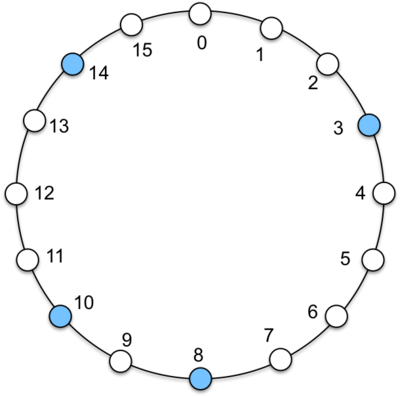
\includegraphics[scale=0.5]{dht-chord-ring.png}
	\caption{Tabla Hash distribuida.}
\end{figure}\\
En la figura por ejemplo se observan como nodos los círculos pequeños. Aquellos que están en azul podrían representar los nodos que son puntos introductorios para algún servicio. Como se observa están bien distribuidos y cubren de manera uniforme el espacio.\\
Para que la red sea lo más dinámica posible y difícil de monitorizar se hace que todas estas posiciones que se le asignan tanto a los nodos como a los servicios ocultos cambien cada 24 horas lo que hace que un nodo o servicio a lo largo de su vida difícilmente esté en una posición en la que ya haya caído previamente.\\
Se estima que hay unos 80 mil servicios ocultos dentro de la red Tor pero sólo 8 mil de ellos son permanentes. La razón de esto es que la mayoría de ellos están dedicados a actividades ilegales o a comunicación entre miembros de bandas organizadas y permanecen la mayoría del tiempo offline para sólo conectarse cuando requieren de comunicación o de ofrecer sus servicios a alguien. Esto hace que sea difícil su vigilancia ya que cambia tanto su posición dentro de la red Tor como su link .onion y sus puntos introductorios.
\subsection{Descriptores en la red Tor}
Los descriptores son documentos que almacenan información de importancia acerca de los nodos en la red Tor. Estos documentos ayudan a la elección de nodos en la red, a saber si es un servicio oculto o cuál es la configuración de dicho nodo. Estos documentos son públicos y como tal pueden ser leídos por cualquiera. Los archivos correspondientes a los nodos son albergados por las Autoridades de Directorio que controlen la parte de la red Tor a la que pertenezca dicho nodo.\\
Los tipos de descriptores que hay dentro de la red son:\\
\begin{itemize}
	\item Server Descriptor: este fichero contiene la información principal de los repetidores. Entre otras cosas se pueden obtener de los mismos sus políticas de salida, ancho de banda, dirección IP, su puerto de conexión OR, sistema operativo,etc. Este fichero es el que un usuario de la red descarga a la hora de decidir los nodos que van a participar en su circuito.
	\item ExtraInfo Descriptor: en este fichero ya se ofrece la información completa del nodo así como sus ficheros de configuración. Este archivo no es descargado por los usuarios por el aumento considerable de tamaño. Aún así, si queremos que nuestro cliente de Tor reciba la información completa de los nodos, podemos configurarlo para ello y en vez de descargarse el fichero Server Descriptor accederá al ExtraInfo Descriptor.
	\item Micro Descriptor: si en vez de utilizar el fichero de Server Descriptor que puede resultar lento en versiones actualizadas del navegador el cliente ya no descarga el archivo Server Descriptor sino Micro Descriptor. Este es básicamente una versión simplificada del original con la intención de que se intercambie menos información al inicio de la comunicación del usuario con la red Tor.
	\item Network Status Document: las Autoridades de Directorio son las encargadas de generar estos ficheros que contienen una valoración de un nodo hecha por las Autoridades. Este fichero es el llamado fichero de consenso que es crucial para el buen funcionamiento de la red ya que no sólo califica la velocidad y configuración sino las posibles intenciones maliciosas del nodo. Este fichero es actualizado con periodicidad para comprobar la integridad de la red a lo largo del tiempo. Los Network Status Documents están compuestos a su vez de ficheros Router Status Entry.
	\item Router Status Entry: estos ficheros incluyen la información sobre cada uno de los repetidores de la red. La información de estos ficheros es proporcionada por cada una de las Autoridades de Directorio de la red. En estos ficheros podemos encontrar los flags que se le van a asignar a los nodos y los cálculos heurísticos de selección de nodos a la hora de formar circuitos.
	\item Hidden Service Descriptor: es el documento que identifica a un servicio oculto. Este fichero es firmado y publicado por el mismo servicio oculto para garantizar la seguridad de la información. Estos documentos son facilitados a los nodos con el flag HSDir que se encargarán de ser asignados como puntos introductorios. Dentro del fichero hay información acerca de la comunicación con el servidor (obtención del punto rendezvous), configuración del servicio oculto, etc.
\end{itemize}
\subsection{Puentes}
Como ya comentamos al principio la red Tor tiene como objetivo principal el hecho de anonimizar a  la persona cuando navega por internet y permitir el acceso seguro a la red incluso en países que filtren algunas webs o todas. A colación de esta pregunta surge un problema de diseño de la red. Si los nodos publican toda su información incluyendo su ip, entonces simplemente con bloquear una gran parte de nodos de la red Tor o la mayoría de los nodos de entrada o salida ya estaremos filtrando el acceso a la red de los usuarios. Este problema a día de hoy ya está resuelto y a dicha solución se la conoce como puentes o bridges en inglés.\\
Un puente dentro de la red Tor es un nodo de acceso a la red que no publica su información y cuya ip va variando cada cierto tiempo. Esto hace que en un principio estos nodos no se puedan bloquear porque no se conoce su información, y aún sabiendo la ip esta cambiará cada cierto tiempo haciendo que cualquier lista negra se quede obsoleta.\\
Esta idea de oscurecer los nodos es un buen comienzo, pero, ¿cómo se conocen por tanto las ips de los nodos para poder configurar nuestra conexión a Tor? La solución dada de momento es consultar una base de datos que proporciona una ip por usuario que solicite un puente. Si la página web que soporta dicha base de datos también está bloqueada en el país del usuario, entonces existe un correo electrónico que interpreta comandos enviados mediante e-mail y devuelve las ips de los puentes solicitados.\\
Gracias a esta solución actualmente países como China, Afganistán o Siria pueden utilizar la red Tor para comunicarse con el exterior.
\subsection{Directorios Tor o Autoridades de Directorio}
Las Autoridades de Directorio en la red Tor son unos servidores encargados de la gestión, mantenimiento y ordenación de los nodos en la red y su información. Estos servidores son los únicos en los que la red confía y son todos ellos pertenecientes a los creadores del proyecto. Precisamente por estos servidores se dice que Tor es una red parcialmente descentralizada, ya que estos ordenadores suponen la parte centralizada de la misma. Actualmente hay 10 autoridades de directorio, siendo dicho número variable a lo largo del tiempo para mantener la capacidad de la red.\\
Las autoridades de directorio han sufrido varios cambios a lo largo del tiempo que han conformado lo que son actualmente:
\begin{itemize}
	\item Versión 1:
		En esta versión las autoridades de directorio se concibieron como servidores a los que se les pedía información sobre los descriptores de los nodos. A raíz de esta funcionalidad se creó la caché de directorio que agiliza la consulta sobre nodos de la red.
	\item Versión 2:
		En esta versión se agilizó un poco más la consulta sobre nodos a las autoridades de directorio, ya que desde esta versión los usuarios sólo descargan la información de los nodos cuya información no conocen. Así mismo se implementó el "network status" el cual es actualizado cada hora y que indica el estado de la porción de la red que controla una Autoridad de Directorio.
	\item Versión 3:
		En esta última versión se mejora el uso de la banda ancha como en las anteriores. Además se introduce el consenso de los network status y las votaciones de las autoridades. En consenso de los network status es un archivo que almacena la información de los nodos que han conseguido pasar la votación de los nodos, es decir, que cumplen las características necesarias para ser usados en la red. El proceso de votación consiste en el voto de cada una de las autoridades acerca de los nodos que se incluyen en su porción de red. Con estos datos el consenso de network status es rellenado para obtener todos los nodos válidos. De este consenso se almacenan las tres últimas versiones para no descartar nodos tan drásticamente.
\end{itemize}
\subsection{Vulnerabilidades teóricas y reales encontradas en Tor}
Tor, aún siendo una buena propuesta de seguridad y anonimato, no es una red segura por completo. Hay ciertas vulnerabilidades de seguridad importantes que sufre la red Tor, ya sea de manera real o teórica. A continuación vamos a presentar algunos ataques y vulnerabilidades que sufre la red Tor.

\subsubsection{Correlación de punto a punto}
Tor ha montado una red completa para el uso desde el exterior, es decir, el uso desde el internet general. La seguridad de Tor recae sobre la propia red y no sobre sus fronteras, por lo que en los extremos de la red Tor nosotros podemos monitorizar el tráfico.\\
Supongamos que somos capaces de controlar nodos de la red Tor y tuviéramos en nuestro poder un número importante de nodos tanto de entrada como de salida. La idea que surje es clara, el nodo de entrada conoce la identidad de la persona y el nodo de salida conoce la información de la comunicación. Aquí es donde podemos intentar establecer una correlación entre la información de entrada y la información de salida. Por ejemplo a través de identidades con las que nos conectemos a servicios por medio de la red Tor o por el contenido en general de los paquetes de red enviados y filtrados en el nodo de salida.\\
Esta técnica se dice que ya ha sido utilizada por agencias como la NSA para el control de la pedofilia, tráfico de armas, tráfico de droga y trata de personas a través de la red Tor. Aunque esta vulnerabilidad existe no es un ataque inexpugnable. La protección ante este ataque podría ser, por ejemplo, el uso de un servicio oculto de la red Tor. Con este servicio el tráfico nunca sale de la red y por tanto la comunicación permanece segura.

\subsubsection{Pérdida de información del nodo de salida}
Como ya hemos comentado anteriormente una de las partes más críticas de la red Tor son los nodos de salida. En concreto este ataque se basa en una de las cosas dichas anteriormente en las características de los nodos de salida. La información en los nodos de salida no va encriptada por lo que, si tenemos un nodo Tor alojado en nuestro ordenador y este nodo consigue el flag de salida exit podemos analizar todo lo que enviamos a la red.\\
El potencial problema de este ataque recae en que se pueden obtener credenciales de inicio de sesión de los servicios a los que el cliente esté intentando acceder. Este ataque fue descubierto por Dan Egerstad que fue capaz de  obtener los credenciales de cuentas de correo electrónico de usuarios de la red Tor empleando este método.

\subsubsection{Bloqueo de nodos de salida}
Este problema no es en realidad una vulnerabilidad de la red Tor en cuanto a seguridad sino un problema de diseño de la misma. El proyecto se ha preocupado por las personas que quieran acceder a la red Tor y tengan los nodos de entrada bloqueados o filtrados (en su empresa, país o por su ISP) mediante los puentes. Este problema plantea justo la misma situación pero con los nodos de salida. Por ejemplo, páginas de ciertos estados o bancos no son accesibles desde la red Tor porque las IPs de los nodos de salida son bloqueadas por dichas empresas. Este problema hace por tanto que en ciertas circunstancias o en ciertas webs la red Tor no sea utilizable.

\subsubsection{Filtración de identidad a través de BitTorrent}
En este caso tenemos dos perspectivas del problema: el "Bad Apple Attack" y la exposición de IPs.\\
En la primera perspectiva algunos investigadores se dieron cuenta de que utilizando BitTorrent dentro de la red Tor con una aplicación no segura y no preparada para el uso de Tor se podía descubrir la IP del usuario de la aplicación de BitTorrent. Esta aplicación intentará conectarse al ordenador "Bad Apple" para descargar un fichero o compartirlo y cederá su IP al atacante. Con este ataque quedó expuesto casi el 40$\%$ del tráfico de la red Tor que precisamente consiste en compartir ficheros mediante torrent.\\
En la segunda perspectiva se va aún más lejos permitiendo, gracias a la recopilación de IPs con el método anterior, hacer un secuestro de sesión o un Man in the Middle pudiendo así atacar al usuario de torrent. Esto como ya he mencionado antes hace que la transmisión de ficheros por la red Tor no sea totalmente segura pudiendo saltarse con ello las protecciones y filtros de anonimato de Tor.

\subsubsection{Ataque DDOS a Tor}
El ataque de denegación de servicio es algo a lo que ni siquiera Tor escapa. Este ataque, como ya es conocido, intenta mediante peticiones masivas interrumpir el funcionamiento de un servidor o en este caso de un nodo de la red. Al ser la información de la red Tor pública se pueden obtener las IPs de los nodos de manera simple y por tanto, si se tuvieran las suficientes máquinas para hacer dicho ataque, se podría cortar el servicio de muchos o todos los nodos de la red haciendo por tanto que no funcione. Este ataque se podría particularizar sobre los nodos de entrada o salida y con ello ya quedaría  inutilizada. El mecanismo de protección de Tor ante esto es el dinamismo de los nodos de salida y entrada (cambian con frecuencia) y el número tan amplio de nodos a los que se debería de atacar para interrumpir el servicio.

\subsubsection{HeartBleed}
Esta conocida vulnerabilidad de SSL sobre HTTPS afectó también a la red Tor que estuvo varios días sin ofrecer servicio mientras renovaba todas sus claves y todos sus certificados con la intención de invalidar la posible información que los atacantes hubieran obtenido. Este ataque sigue siendo aplicable si hay aún alguna web HTTPS que no tenga el parche de seguridad que arregló la vulnerabilidad.
	
\newpage

\section{Riffle como solución}
\subsection{Introducción. Comparaciones}
El anonimato es un derecho fundamental en toda sociedad democrática y es crucial en la libertad de expresión. Las redes anónimas como Tor, ya presentado anteriormente, han ido ganando popularidad en los usuarios interesados en altos niveles de privacidad. Sin embargo, estos sistemas son susceptibles ante ataques basados en análisis de tráfico, llevados a cabo por poderosos adversarios como estados autoritarios o que controlan los ISP, o incluso adversarios menores que han sido capaces de controlar el tráfico de los usuarios.
Existen dos tipos de redes que ofrecen resistencia al análisis del tráfico incluso bajo la presencia de tales adversarios. Son las DC-Nets (Dining-Crytographer Networks), donde la red está formada por servidores y clientes y se preserva el anonimato si se asegura la existencia de un servidor honesto (no malicioso) , y las MixNets, o redes mixtas, que usan mezclas verificables para permutar los textos cifrados de forma que se mantiene la privacidad. Sin embargo, ambas dos presentan problemas de eficiencia. La primera, sufre un gran overhead de banda ancha para poder garantizar la privacidad, y la segunda, un gran overhead computacional. 

Es por eso que presentamos Riffle como alternativa. Riffle es un sistema de comunicación anónima que garantiza una férrea resistencia al análisis del tráfico y una fuerte privacidad minimizando los costes computacionales y de banda ancha, dando lugar a un sistema altamente eficiente. Para ello, aglutina una serie de ideas innovadoras tales como:

\begin{itemize}
	\item Un sistema híbrido de mezcla garantizada que usa encriptación simétrica, evitando la costosa mezcla de claves públicas.
	\item Una nueva aplicación de recuperación de información privada.
	\item Una gran eficiencia en las comunicaciones anónimas resistentes tanto a los análisis de tráfico como a los clientes maliciosos.
\end{itemize}

\textbf{\large{Propiedades de Seguridad}} \\ 

Riffle posee tres propiedades de seguridad principales. La primera es corrección, que garantiza que Riffle es un sistema de comunicación válido.

\textbf{Definición 1.} \textit{El protocolo es correcto si, después de una ejecución satisfactoria del protocolo, todo mensaje de un cliente honesto está disponible para todos los clientes honestos.} \\

Además, Riffle pretende proveer de dos propiedades de anonimato más: anonimato del emisor y del receptor. \\

\textbf{Definición 2.} \textit{El protocolo provee anonimato al emisor si, para toda ronda de comunicación, la probabilidad de que un adversario descubra el cliente honesto que mandó un mensaje es suficientemente cercana a 1/k, siendo k el número de clientes honestos.} \\

Es decir, que ningún adversario puede franquear el anonimato de un cliente honesto. La privacidad del receptor es totalmente complementaria: \\

\textbf{Definition 3.} \textit{El protocolo provee anonimato al receptor si, para toda ronda de comunicación, la probabilidad de que un adversario descubra cuál de los n mensajes ha recibido un cliente honesto es suficientemente cercana a 1/n, donde n es el número de mensajes disponibles.}  \\

En el caso de los receptores, los clientes no producen ningún mensaje, así que la única información disponible para un adversario son los metadatos, los cuales serán ocultos tanto como sea posible.
\subsection{Arquitectura Riffle}
Esta sección comienza con un protocolo base que nos introduce en la estructura de Riffle pero con ciertos problemas de seguridad e ineficiencia. A continuación presentamos las primitivas criptográficas usadas en Riffle y el protocolo final. Finalmente haremos un breve estudio del overhead de banda ancha y un análisis de seguridad

\subsubsection{Primer acercamiento: Protocolo base}
Esta será la base del protocolo de Riffle. Este protocolo se lleva acabo en $"$épocas$"$ o etapas, y cada una de ellas está formada por dos fases: configuración y comunicación. La fase de configuración se usa para compartir claves y ocurre sólo una vez en el inicio de cada etapa. La fase de comunicación consta de múltiples rondas, y los clientes descargan y mandan mensajes a los servidores en cada una de ellas.

Durante la etapa de configuración, cada servidor $S_i$ genera una clave pública $p_i$, y todas las claves se hacen publicas para todos los clientes y servidores del grupo. Cada ronda de la fase de comunicación consta de tres etapas: (1) subida, (2) mezcla, y (3) descarga. En la fase de subida, un cliente $C_j$ encripta por capas (onion-encrypting) su mensaje con todas las clave públicas $\{p_i:i \in [1,m]\}$ y sube dicho texto cifrado a su servidor principal. Cuando todos los textos cifrados se han subido, el primer servidor $S_1$ recopila los textos. 

En la etapa de mezcla, encabezada por el servidor $S_1$, los servidores llevan a cabo una mezcla y desencriptación fiable. Cada servidor manda la prueba de la desencriptación y permuta, repartiéndolos, los textos desencriptados entre todos los demás servidores., los cuales verifican las pruebas recibidas. Este proceso de desencriptación, mezcla y verificación de las pruebas se repite hasta que el último servidor revela todos los textos planos, sin encriptación, a todos los servidores.

Finalmente, en la etapa de descarga, todos los mensajes en texto plano se difunden a los clientes a través del servidor principal de cada cliente. 

\subsubsection{Mezcla híbrida comprobable}

A pesar del ahorro significativo de banda ancha, el exceso de costes computaciones de las mezclas fiables que lleva a cabo el protocolo base hace que sea inapropiado para comunicaciones con gran banda ancha. Para abordar y mejorar los aspectos de la mezcla comprobable tradicional, proponemos una nueva mezcla híbrida, la cual se lleva a cabo una sola vez para compartir las claves encriptadas que se usan durante una época. Utilizamos encriptación autenticada en las claves compartidas y verificamos las mezclas a través de textos cifrados autenticados. Intuitivamente, se impulsa la verificación de la mezcla inicial de las claves.

La mezcla, o permutación, puede ser descrita como un protocolo llevado a cabo por tres conjuntos disjutos: los clientes, un servidor probador y un servidor verificador. El objetivo del cliente es mandar R conjuntos de n mensajes al verificador usando el probador, siempre que se satisfagan dos propiedades. La primera, que el verificador no sabe el orden de los mensajes en cada conjunto. La segunda, el verificador debe poder comprobar si el probador alteró o borró algún mensaje. A continuación, se expone el algoritmo. \\

\textbf{Algoritmo 1. Mezcla híbrida}
\begin{enumerate}
	\item \textbf{Compartir claves:} Un probador P y un verificador V generan parejas de claves públicas-privadas $(s_P,p_P)$ y $(s_V,p_V)$ y hacen públicas las claves $p_P$ y $p_V$. Un cliente C comparte sus claves $\{k'_i: i \in [n]\}$ con P.
	\item \textbf{Permutación de las claves:} C genera $\{k_i: i \in [n]\}$ para V y manda $\{Enc_{p_p}(Enc_{p_v}(k_j))\}$ a P y V. P desencripta y mezcla de
	forma verificada usando una permutación aleatoria $\pi$, y manda
	$\{Enc{p_v}(k_{\pi_j})\}$ a V. V verifica la mezcla y la desencriptación, y desencripta para ver $\{k_{\pi _j}\}$.
	\item  \textbf{Envío de mensajes:} Para $r=1,...,R,$
	\begin{enumerate}
		\item Mezcla: Para mandar mensajes $\{M_j^r\}_{j \in [n]}$ C encripta los mensajes en capas (onion-encrypt) y envía
		 $\{AEnc_{k'_j,r}(A Enc_{k_j ,r}(M_j ^r))\}_{j \in [n]}$ a P, donde $AEnc$ es un esquema autenticado encriptado que usa r como nonce. P desencripta una capa de la encriptación usando $\{k'_j\}_{j \in [n]}$, los permuta usando la misma $\pi$ y manda $\{AEnc_{k_\pi(j),r}(M_{\pi(j)} ^r))\}_{j \in [n]}$ a V.
		 \item Verificación: V verifica el texto cifrado comprobando la autenticación a través de las claves $\{k_{\pi(j)}\}_{j \in [n]}$ y r, desencripta una capa y adquiere los mensajes $\{M_{\pi(j)}^r\}_{j \in [n]}$.
	\end{enumerate}
	
\subsection{Recuperación de información privada (PIR) en Riffle}
Existen situaciones en las que un cliente no está interesado en la mayoría de los mensajes. Por ejemplo, consideremos dos clientes
chateando a través de Riffle. Si los mensajes se mezclan usando la misma permutación cada ronda, los clientes pueden intuir la localización de los mensajes tras una ronda de comunicación, pero para leer los propios
están obligados a descargar todos los mensajes disponibles. En este escenario, podemos usar el multiservidor de recuperación de información privada (PIR), propuesto para mejorar la eficiencia en la comunicación. 
Veamos cómo funciona: sea $I_j$ la localización (índice) del mensaje que el cliente $C_j$ quiere acceder. Para descargar el mensaje, $C_j$
primero genera m-1 máscaras de bits aleatorias de longitud n, y computa cada una de forma que la XOR de todas las m máscaras da lugar a una máscara con un 1 sólo en la posición $I_j$. Cada máscara se manda a un servidor y cada servidor $S_i$ hace la XOR a los mensajes en las posiciones con 1 en la máscara para generar las respuestas $r_{i,j}$ para $C_j$. Finalmente, $C_j$ descarga todos los $\{r_{i,j}\}_{i \in [m]}$ y les hace la XOR a todos juntos para adquirir el mensaje en texto plano. 
Aunque este algoritmo es muy eficiente, se puede reducir aún más el overhead de banda ancha usando generadores de números pseudoaleatorios (PRNGs). Para evitar mandar las máscaras a todos los servidores en cada ronda, $C_j$ comparte una máscara inicial con todos los servidos en la fase de configuración. Cada servidor actualiza después la máscara internamente por medio de un PRNG cada ronda, de forma que $C_j$ solo manda una máscara a su servidor principal $S_{p_j}$ para asegurar que la XOR de todas las máscaras tienen un 1 solamente en la posición $I_j$

Para evitar la descarga de un mensaje en cada servidor, $C_j$ puede pedirle a $S_{p_j}$ que recoja todas las respuestas y le haga la XOR a todas juntas. Sin embargo, si se hace eso, el servidor principal de $C_j$ conocería el mensaje que $C_j$ quiere descargar. Para prevenir este problema, $C_j$ comparte otra serie de secretos con cada servidor durante la configuración, y cada servidor hace la XOR del secreto en la respuesta. $S_{p_j}$ ahora puede recoger las respuestas y hacerles la XOR sin saber nada sobre el mensaje. Finalmente, $C_j$ descarga la respuesta de $S_{p_j}$ (es decir, el mensaje XOR con los secretos compartidos) y borra los secretos para recuperar el mensaje. 

\textbf{Algoritmo 2. Recuperación de información privada}
\begin{enumerate}
	\item Configuración. Cada cliente $C_j$ comparte dos secretos $m_{i,j}$ y $s_{i,j}$  con cada servidor $S_i$ excepto con su servidor principal $S_{p_j}$. Esto pasa una vez por época.
	\item Descarga:
	\begin{enumerate}
		\item Generación de máscaras. Sea $I_j$ el índice del mensaje que $C_j$ quiere descargar. $C_j$ genera $m_{p_j,j}$ de forma que $\oplus _i m_{i,j} = e_{I_j}$, donde $e_{I_j}$ es una máscara de bits con un 1 en el índice $I_j$. $C_j$ manda $m_{p_j,j}$ a $S_{p_j}$.
		\item Generación de la respuesta. Cada servidor $S_i$ computa la respuesta $r_{i,j}$ para $C_j$ calculando la XOR de los mensajes en las posiciones donde hay 1's en $m_{i,j}$, y haciendo la XOR a los $s_{i,j}$. Específicamente, $r_{i,j} = (\oplus _l m_{i,j}(l) \land M_l) \oplus s_{i,j}$, donde $M_l$ es el mensaje en este plano número $l$. Entonces, los servidores mandan $r_{i,j}$ a $S_{p_j}$ y éste calcula $r_j$:
		$r_j=\oplus _i r_{i,j} = (\oplus _i \oplus _l m_{i,j}[l] M_l) \oplus (\oplus _i s_{i,j}) = M_{I_j} \oplus (\oplus _i s_{i,j})$.
		\item Descarga del mensaje. $C_j$ descarga $r_j$ de $S_{p_j}$ y hace la XOR de todos los $\{s_{i,j}\}_{i \in [m]}$ para obtener el mensaje deseado, $M_{I_j}= r_j \oplus (\oplus _i s_{i,j})$.
		\item Actualización de secretos. C y S aplican PRNG a sus máscaras y secretos para refrescarlos. 
	\end{enumerate}
\end{enumerate}

\subsection{Protocolo Riffle}
Presentamos por fin el protocolo Riffle al completo. Durante la fase de configuración, los clientes comparten tres conjuntos de pares secretos con los servidores: (1) $\{k_{i,j}\}$ usando mezcla híbrida y (2) $\{m_{i,j}\}$ y (3) $\{s_{i,j}\}$ usando PIR. Cada servidor genera una permutación $\pi_i$ para la mezcla verificada y las retienen para su futuro en uso en la fase de comunicación. Las claves $\{k_{i,j}\}$ estarán en la posición $\pi_i-1(...(\pi(j))...)$ en $S_i$ al final de la configuración. 

En la ronda $r$ de la fase de comunicación, el protocolo usa la mezcla híbrida para subir datos y PIR para descargar. En la etapa de subida, cada cliente $C_j$ encripta por capas un mensaje usando $\{k_{i,j}\}_{i \in [m]}$ y sube los textos cifrados al servidor $S_1$ a través de su servidor primario. En la etapa de mezcla, empezando por $S_1$, cada $S_i$ autentica y desencripta los textos cifrados utilizando las mismas claves $\{k_{i,j}\}_{i \in [m]}$, las mezcla usando $\pi_i$ guardada en
la fase de configuración, y envía el resultado al siguiente servidor. 
Esto implica que en $S_i$, el texto cifrado $A Enc_{k_{i,j},r}(...(A Enc_{k_{mj},r}(M_j ^r))...)$ de $C_j$ está en la posición
$\pi_i-1(...(\pi(j))...)$. El último servidor revela los mensajes en texto plano a todos los servidores. La permutación final de los mensajes es $\pi = \pi_m(\pi_{m-1}(...(\pi_2(\pi_1))))$.

En la etapa de descarga, los clientes llevan a cabo un PIR con las máscaras y los secretos, o descargan todos los mensajes a través de difusión.

\textbf{Algoritmo 3. Procolo Riffle}
\begin{enumerate}
	\item Configuración.
	\begin{enumerate}
		\item Mezcla de las claves:
		\begin{enumerate}
			\item Cada servidor $S_i$ genera pares de claves públicas-privada y facilita la pública $p_i$ a los clientes. Además, genera la permutación $\pi_i$.
			\item Cada cliente $C_j$ genera las claves $k_{i,j}$ para $S_i$ y las encripta con las claves $p_1,...,p_i$ para $i=1,...,m$. $C_j$ entrega $m$ $\{k_{i,j}\}$ encriptadas por capas a $S_1$ a través del servidor principal.
			\item Desde $S_1$ a $S_m$, $S_i$ desencripta las claves. $S_i$ las guarda, realiza una mezcla verificada de las otras claves usando $\pi_i$ y las envía mezcladas a $S_{i+1}$, Los servidores verifican la desencriptación y mezclan.
		\end{enumerate}
		\item Compartir secretos: Cada pareja $S_i,C_j$ genera una pareja de secretos $m_{i,j}.s_{i,j}$ utilizados en PIR (Algoritmo 2), en la etapa de descarga.
	\end{enumerate}
	\item Comunicación. En la ronda $r$,
	\begin{enumerate}
		\item Subida de datos. $C_j$ encripta por capas el mensaje $M_j ^r$ usando encriptación autenticada con $\{k_{i,j}\}$ y $r$ como un nonce: $AEnc_{1,...,m}(M_j ^r) = A Enc_{k_{i,j},r}(...(A Enc_{k_{mj},r}(M_j ^r))...)$. $C_j$ entonces envía $AEnc_{1,...,m}(M_j ^r)$ a $S_1$ a través de su servidor principal.
		\item Mezcla. Desde $S_1$ hasta $S-m$, $S_i$ autentica, desencripta y mezcla los textos cifrados usando $\pi_i$, y envía mezclado $\{AEnc_{i+1,...,m}(M_j ^r)\}_{j \in [n]}$ a $S_{i+1}$. $S_m$ comparte los mensajes finales en texto plano con todos los servidores.
		\item Descarga. Los clientes descargan los mensajes en texto plano utilizando PIR.
	\end{enumerate}
\end{enumerate}
	
\end{enumerate} 

\subsection{Acusación}
En redes DC es fácil realizar un ataque de denegación de servicio a la red completa por parte de un cliente malicioso. De hecho, cualquier cliente puede hacer XOR sobre unos bits arbitrarios y corromper un mensaje en cualquier momento. Este problema tiene soluciones complicadas y a veces costosas, como redes trampa o limitar el tamaño del grupo para minimizar los ataques.

Sin tomar algunas precauciones, podemos encontrar ataques como estos en Riffle: durante la subida de datos, un cliente malicioso podría mandar un texto cifrado mal autenticado, de forma que el sistema se detendría. Sin embargo, las mezclas descritas no permiten que la entrada de un cliente corrompa las demás entradas. Teniendo en cuenta esta ventaja, Riffle ofrece una manera eficiente de mantener un cliente responsable sin introducir costes operacionales y sin robar privacidad a los clientes honestos: cuando un servidor $S_i$ detecta que un texto cifrado en la posición $j$ está mal autenticado, inicia el proceso de acusación revelando $j$ a $S_{i-1}$. $S_{i-1}$ revela $j'=\pi_{i-1} ^-1(j)$ y así sucesivamente hasta $S_1$, que revela el cliente que mandó el texto cifrado.

Un cliente malicioso, sin embargo, no puede llevar a cabo el mismo ataque durante la descarga. Cuando los mensajes se difunden, no hay ningún cliente que pueda interrumpir la comunicación. Cuando los clientes usan PIR para descargar el mensaje, no hay una noción de texto cifrado mal autenticado o mensajes "ilegales" que hagan que el sistema se detenga, dado que las máscaras y los secretos son números aleatorios. Además, al igual que en la etapa de subida, un cliente malicioso no puede corromper otros mensajes de clientes dado que cada cliente genera sus propias máscaras y secretos. 

\subsection{Análisis de seguridad}

\subsubsection{Seguridad de la mezcla híbrida}

Necesitamos demostrar dos propiedades de la mezcla: (1) verificabilidad y (2) conocimiento-cero. Para mostrar la primera, asumamos que la encriptación autenticada usada por Riffle es segura ante falsificaciones. Entonces, para que un probador P falsifique sus entradas y no sea detectado por un verificador V, P necesita generar salidas de forma que algunas de ellas no sean desencriptadas de las entradas, pero que se autentiquen de forma adecuada bajo la clave de P. Sin embargo, los textos cifrados son infalsificables y las claves de V son desconocidas dado que P sólo conoce las encriptadas $k_i$. Eso implica que P no puede generar salidas. Utilizamos también el número de ronda, que es cedido internamente por P, como el nonce de la encriptación autenticada para garantizar la originalidad de los datos y detiene ataques repetidos por P. Por tanto, la mezcla y desencriptación de P es valida si y sólo si V puede autenticar todas las salidas de textos cifrados y la mezcla puede ser verificada. 

Para probar el conocimiento-cero, asumimos que el esquema de encriptación es seguro. Eso significa que V sólo aprende información insignificante observando las entradas y salidas de textos cifrados de P. Entonces, V puede simular las respuestas de P encriptando valores aleatorios con las claves almacenadas en V: las claves se guardan en el mismo orden de salida de P, y los textos cifrados salida de P son indistinguibles para la encriptación de valores aleatorios si dicha encriptación es semánticamente segura. Finalmente, las claves en V no filtran la permutación de P dado que la mezcla verificada usada para compartir las claves tiene la propiedad de conocimiento-cero. 

\subsubsection{Seguridad de Riffle}
\begin{itemize}
	\item \textbf{Corrección.} Si el protocolo se completa de forma fidedigna, entonces los servidores simplemente mezclarán los mensajes y el servidor final los publicará en texto plano en todos los servidores. Los mensajes estarán también disponibles para los clientes vía PIR o difusión. 
	\item \textbf{Anonimato del emisor.} El anonimato del emisor se basa en la verificabilidad y conocimiento-cero de la mezcla híbrida. Durante las etapas de subida y mezcla del protocolo. $S_i$, un servidor de subida, es el probador P, y $S_{i+1}$, un servidor de bajada, es el verificador V de la mezcla híbrida. Intuitivamente, verificabilidad asegura que el protocolo se completa fielmente; en caso contrario el servidor honesto notificará un error. Más aún, dado que la mezcla se caracteriza por ser conocimiento-cero, la permutación de un servidor honesto es desconocida para un adversario. Por tanto, la permutación final de los mensajes es también desconocida para un adversario, y ningún cliente o servidor malicioso pueden adquirir un mensaje de otro honesto. 
	\item \textbf{Anonimato del receptor.} El anonimato de las descargas depende de la seguridad del PIR y PRNGs. Intuitivamente, 
	si las máscaras se generan de forma aleatoria, entonces la máscara m-ésima no puede ser inferida de las anteriores. La optimización para reducir el número de veces que se comparten las máscaras es seguro si el PRNG es criptográficamente seguro, lo que quiere decir que las máscaras no se pueden distinguir de máscaras realmente aleatorias. Finalmente, la recopilación de los mensajes en un servidor es segura si los servidores maliciosos no conocen todos los secretos. Si es así, los adversarios no podrían saber el índice del mensaje descargado por un cliente honesto.
\end{itemize}
\newpage

\subsection{Intercambio anónimo de ficheros. Protocolo}
\begin{figure}[h]
	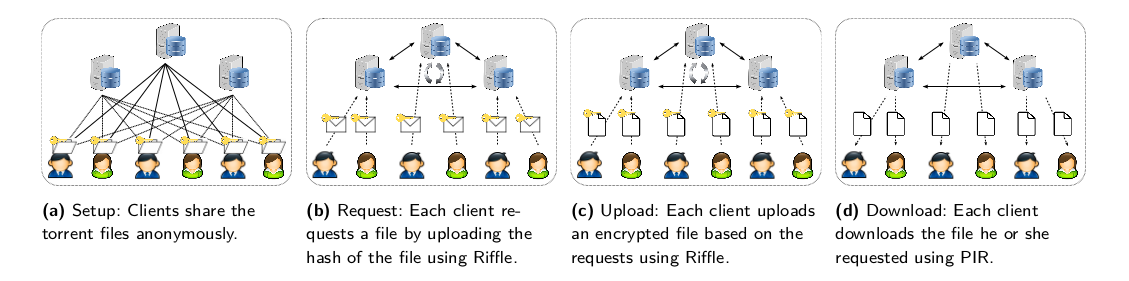
\includegraphics[scale=0.2]{anonymous.png}
	\caption{Protocolo de transferencia de archivos anónimo}
\end{figure}

\subsubsection{Protocolo de compartición de archivos}

La manera de compartir archivos en un grupo Riffle es similar a como lo hace BitTorrent, a pesar de las diferencias en el modelo (BitTorrent utiliza peer-to-peer y Riffle cliente-servidor). CUanod un cliente quiere compartir un archivo, genera un torrent, que contiene los hashes de todos los bloques del archivo. Entonces, usando Riffle, el cliente sube el torrent al servidor. Los servidores toman el papel de rastreador de torrentes en BitTorrent, y gestionan todos los archivos disponibles en el grupo. En el diseño más simple, los descriptores de archivo se difunden a todos los clientes conectados, y pueden elegir localmente un archivo para descargarlo. Dado que los torrent son suficientemente pequeños, incluso para archivos grandes, y compartirlos no es apenas costoso, asumimos que difundirlos no tiene ningún coste y nos centramos en compartir bloques. 

Con los torrents distribuídos, los clientes pueden ahora compartir de forma anónima los archivos usando Riffle. Este hecho se da en tres pasos:
\begin{enumerate}
	\item \textbf{Petición de bloques}. Cada $C_j$ identifica un archivo F de su interés y los hashes de los bloques del archivo $H_F$ a través del torrent. $C_j$ solicita un bloque de F subiendo el hash de dicho bloque a su servidor principal $S_{p_j}$ usando Riffle. Cuando un cliente no necesita requiere ningún bloque, manda un valor aleatorio como seña de que no quiere nada. Todas las peticiones $H_\pi$ se difunden a los clientes al final de este paso.
	\item \textbf{Subida de bloques.} Cada $C_j$ comprueba si tiene algún bloque mirando los hashes de los bloques que posee. Si encuentra alguno, entonces lo sube usando Riffle. Una vez que el texto plano del bloque está disponible para los servidores, cada servidor difunde los hashes $H'_\pi$ que tiene a su alcance a todos los clientes.
	\item \textbf{Descarga de bloques.} Desde $H_\pi$ y $H'_\pi$, $C_j$ conoce el índice del bloque pedido. Usando PIR, $C_j$ descarga el bloque. 
\end{enumerate}	

	Cada una de las peticiones son independientes, así que se pueden dar de forma paralela. En la figura 2 se resume el protocolo.

\subsubsection{Costes de banda ancha en la compartición de archivos}

Para compartir cada bloque entre usuarios en BitTorrent, cada cliente necesita solicitar y descargar un bloque. También podría necesitar subir un archivo si recibe una solicitud. Si cada solicitud tiene tamaño $h$, cada cliente consume $h+b$ de la banda ancha de subida y $b$ de la banda ancha de bajada. En Riffle con PIR, hay tres fuentes de costes de banda ancha por cliente: (1) descargar las peticiones, (2) subir los MACs de encriptación autenticada y (3) las máscaras para el servidor principal.  Por tanto, el total de banda ancha entre un cliente y un servidor es $h+b+n+2m \lambda$ de subida, y $b+2hn$ de bajada. Nótese que aunque la banda ancha necesaria crece con el número de clientes, $n$ y $2hn$ son mucho más pequeñas que $b$ en escenarios de compartición de archivos para un número razonable de clientes y de tamaño de archivo. 

	

\newpage

\section{Demos}
\subsection{Demo de Tor}
La demostración que hemos preparado para Tor ha consistido en montar un nodo tor y mantenerlo en ejecución durante una semana siendo monitorizado con la aplicación de consola ARM.\\
ARM es un monitor de nodos Tor que da información muy valiosa acerca del mismo. Es capaz de decirte los recursos que está consumiendo dicho nodo en la máquina y cuales son las gráficas de uso de la red. Con ello podemos observar que cantidad de información estamos siendo capaces de rediredcionar a través de nuestra red. También nos dice, aunque de manera menos precisa por motivos de diseño de la red Tor, los circuitos en los que estamos participando como nodo así como la configuración de nuestro nodo. Así mismo uno de los campos más importantes y con lo que hemos podido probar y ver nuestro desarrollo teórico de Tor ha sido mediante los flags.\\
Para la configuración del nodo Tor se deben de establecer los parámetros que se deseen en un fichero llamado torrc. Este fichero contiene las directivas de configuración de un nodo Tor cualquiera, entre las cuales están por ejemplo qué puertos usar o cuanta banda ancha ofrecemos para el nodo. En nuestro caso, teníamos que tener precauciones al configurar nuestro nodo de prueba. En la red Tor aunque no se quiera se mueve mucho contenido altamente ilegal en España como pornografía infantil, contrabando de drogas y armas y comunicaciones de bandas ilegales. Si nuestro nodo hubiera sido un nodo de salida, nuestro ordenador habría sido el encargado de hacer las peticiones y recolectar información de las páginas web con contenidos ilegales para facilitarlos al usuario de Tor, por lo que en términos legales nosotros habríamos sido los que han infligido un acto delictivo. Es por eso que nuestro nodo lo configuramos con la política "reject *:*" la cual indica que se rechaza cualquier puerto de cualquier IP para las funciones de nodo de salida. El resto de configuraciones que hicimos no fueron demasiado complejas ya que la documentación de los archivos torrc está muy bien explicada y su uso es bastante sencillo.\\
Durante nuestro experimento el nodo adquirió los flags V2Dir, Running y Valid. Estos flags como ya explicamos indican que nuestro nodo era compatible con la segunda versión del protocolo de Autoridades de Directorio, que el nodo estuvo en ejecución estable por al menos 45 minutos y que no estábamos ejecutando una versión maliciosa de Tor ni estábamos en ninguna lista negra. Estos flags fueron el fruto de una conexión de unos 100KB/s de subida y 100KB/s de bajada mantenida, como ya hemos dicho, durante 7 días.\\
El monitor ARM es muy expresivo a la hora de comunicarte las comprobaciones que se realizan sobre tu nodo acerca de la velocidad, accesibilidad y adquisición de flags por lo que pudimos observar como nuestro nodo era calificado por las Autoridades. También nos fijamos que cualquier nodo posee un nombre establecido por el usuario que no es identificativo del mismo y un fingerprint que es el usado dentro de la tabla hash interna de la red Tor para manejar los nodos.\\
ARM como ya hemos comentado también da información de los nodos que conforman el circuito aunque dicha información no es precisa. Aún así nos permitió ver cómo son las configuraciones de un nodo Tor de salida o entrada y la variedad de países que participan en el proyecto Tor instalando nodos.\\
Así mismo hemos recurrido a páginas como "Tor status" para ver la actividad de nuestro nodo y qué posición ocupábamos dentro del ranking de nodos. Esta misma página nos permitía comprobar los datos de tráfico de red que nos estaba dando ARM con los que la página nos proporcionaba, viendo así que el nodo funcionaba de manera correcta. Por último para hacer un análisis más general de tor hemos acudido al portal de "Tor metrics" del propio Tor Project. En este portal podemos comprobar datos como cuantos nodos hay activos, cuales son los temas que se encuentran en Tor o los países que más emplean la red entre otras cosas. Como curiosidad también encontramos la web "Tor flow" que proporciona un gráfico mundial del movimiento de información dentro de la red.	
\subsection{Demo de Riffle}
En esta última parte discutimos la implementación y prototipo presentado por los investigadores del MIT.

La implementación está hecha sobre el lenguaje de programación Go. El prototipo se ha basado en dos aspectos: compartición de archivos y un microblog, esto es, cada cliente envía mensajes cortos en texto plano los cuales se difunden a todos los demás usuarios (a la manera de Twitter). Los códigos fuentes son de dominio público. Hemos intentado contactar con los creadores vía email y aún esperamos respuesta, para que nos expliquen, al menos por encima, cómo compilarlo, ejecutarlo y cómo funciona. 

\subsection{Compartición de archivos}
En la implementación de esta parte están incluídos todos los avances descritos previamente. Los archivos utilizados para la prueba están divididos en bloques de 256KB, similar a como lo hace BitTorrent. En los experimentos, Riffle tiene buenos resultados con hasta 200 clientes, soportando 100KB/s de banda ancha efectiva por cliente. La primera restricción que se encuentra es la banda ancha del servidor. Si el servidor estuviera conectado con 10 Gbps, se obtendría un funcionamiento idóneo.
 
 Las discrepancias entre  el modelo ideal y el prototipo para un gran número de clientes es debido a dos factores: primero, el modelo ideal desprecia los costes computacionales, los cuales crecen linealmente con el número de clientes. Aunque la desencriptación no supone grandes costes, estos se vuelven representativos cuando el número de clientes es alto. Finalmente, la banda ancha efectiva (disponible) para cada cliente decrece dado que compartimos 100 Mbps entre algunos cientos de clientes. 
 
 Aunque Riffle parecer ser poco eficiente, protege el anonimato de forma consistente: el prototipo garantiza el anonimato tanto del emisor como del receptor. Las operaciones descritas en los apartados anteriores, como PIR o mezcla híbrida son costosas y algo lentas, dado que están muy orientadas a la seguridad. Sin embargo, los creadores tienen confianza en encontrar formas de ganar eficiencia sin perder de vista este paradigma. 
 
 \subsection{Microblog}
 
 Los creadores han simulado una situación de microblog creando cientos de miles de clientes que mandan un pequeño mensaje (160B hasta 320B) cada ronda, difundiéndolo a todos los clientes al final de cada ronda. Debido a las limitaciones técnicas, han creado cientos de miles de "superclientes" y cada uno de ellos manda cientos de mensajes para simular un gran número de usuarios. Los resultados obtenidos dicen que se pueden soportar 10000 usuarios con menos de un segundo de latencia con mensajes de 160B. Si admitimos algo de latencia entre mensajes, se pueden soportar más de 100000 usuarios con un delay de 10 segundos. Además, se ha visto que la latencia decrece de forma proporcional con mensajes más cortos. Dado que Riffle es eficiente, la latencia se determina solamente con el número total de bits contenidos en los mensajes en cada ronda. Esto facilita la extracción de conclusiones en materia de eficiencia y su relación con el número de usuarios y el tamaño del mensaje. 
 
 
\clearpage
	
% Bibliografía.
%-----------------------------------------------------------------
\onecolumn
\begin{thebibliography}{11}
	
	\bibitem{Cd10}
	\textsc{Kwon, Lazar, Devadas, Ford} \\
	\textit{Riffle}, Proceedings on Privacy Enhancing; 2016 (2):1-20.
	
	\bibitem{Cd11}
	\textsc{Juan Luis García Rambla, Chema Alonso} \\
	\textit{Ataques en redes de datos IPv4 e IPv6}
	
	\bibitem{Cd12}
	\textsc{Daniel Echeverri} \\
	\textit{Deep Web: Tor, FreeNET \& I2P: privacidad y anonimato.}
	
	\bibitem{Cd13}
	\textsc{Documentación Tor Project} \\
	\textit{https://www.torproject.org/docs/documentation.html.en}
	
	\bibitem{Cd14}
	\textsc{Documentación ARM} \\
	\textit{https://www.atagar.com/arm/}
	
	\bibitem{Cd15}
	\textsc{Conferencias Tor} \\
	\textit{Youtube}

	
\end{thebibliography}	
	
	
\end{document}